\newpage
%%%%%%%%%%%%%%%%%%%%%%%%%%%%%%%%%%%%%%%%%%%%%%%%%%%%%%%%%%%%%%%%
%%%%%%%%%%%%%%%%%%%%%%%%%%%%%%%%%%%%%%%%%%%%%%%%%%%%%%%%%%%%%%%%
%%%%%%%%%%%%%%%%%%%%%%%%%% Enunciado %%%%%%%%%%%%%%%%%%%%%%%%%%%

\begin{myblock}
\phantomsection\addcontentsline{toc}{section}{Parte A | Generación de texto}
\section*{Parte A | Generación de texto}

    Reune al menos 100 canciones de tu género de música favorito. Unifica todo en un 
    solo archivo de texto (canciones.txt), separando cada canción con un delimitador claro. 
    Por ejemplo: <|startsong|> y <|endsong|> en una línea. 

    Además, normaliza con codificación UTF-8, elimina ruido (cabeceras repetidas, metadatos, 
    anuncios) y documenta tus decisiones de preprocesamiento.

\end{myblock}

%%%%%%%%%%%%%%%%%%%%%%%%%%%%%%%%%%%%%%%%%%%%%%%%%%%%%%%%%%%%%%%%
%%%%%%%%%%%%%%%%%%%%%%%%%%%%%%%%%%%%%%%%%%%%%%%%%%%%%%%%%%%%%%%%

%%%%%%%%%%%%%%%%%%%%%%%%%%%%%%%%%%%%%%%%%%%%%%%%%%%%%%%%%%%%%%%%
%%%%%%%%%%%%%%%%%%%%%%%%%%%%%%%%%%%%%%%%%%%%%%%%%%%%%%%%%%%%%%%%

Para esta tarea se reunieron canciones de la banda 'Twenty One Pilots'. Entre su discografía
se encuentran más de 100 canciones, que en general combinan composiciones y estructuras
del Hip Hop, Rap Rock, electropop y Synth-pop. En general es una banda que combina distintos
géneros, ritmos y estructuras, pero pensé que mantener un corpus de una misma banda podría
ser interesante. 

Para no descargar de manera manual las canciones, utilizamos la API de Genius. Genius es una 
página web dedicada a la captura y exposición de letras de canciones, así como a la colaboración
con fanáticos de las bandas para interpretar y dar explicación a fragmentos de las canciones. La
API de esta página permite, de manera sencila, acceder a su base de datos para sustraer las
letras que te interesen. Puedes realizarlo por título de canción, o por álbum, así como por artista
artista. La descarga de los datos es relativamente sencilla utilizando Python. 

El proceso de descarga se automatizó mediante un script, utilizando la biblioteca \texttt{lyricsgenius},
la cual funciona como un cliente para la API de Genius. La implementación se dividió en varias
fases clave para asegurar una recolección de datos robusta y limpia. 

Primero, se configuró el acceso a la API con un token de autenticación. Para refinar la calidad
de los datos edsde el inicio, se establecieron parámetros específicos en el cliente de \texttt{lyricsgenius}:

\begin{itemize}
    \item Se excluyeron términos como "Remix" y "Live" para evitar versiones alternativas de 
    las canciones y enfocarse en las letras de estudio.
    \item Se activó la opción \texttt{remove\_section\_headers} para eliminar automáticamente las
    las etiquetas estructurales de las letras (ej. \texttt{[Chorus]}, \texttt{[Verse]}), loaded
    cual representa un primer paso de preprocesamiento. 
\end{itemize}

Además de canciones por álbum se añadieron a la lista de descargas canciones que son sencillos 
de la banda, como 'Heathens' y 'Level of Concern'. Toda la información recolectada, es decir, el título
de la canción, el álbum y la letra, se almacenó en una estructura ed datos utilizando Pandas. 

Como último paso de limpieza en esta sección, se eliminaron posibles entradas duplicadas revisando el título
de las canciones. El resultado fue un corpus consolidado por un archivo en CSV llamado: \texttt{TOP\_lyrics\_hybrid.csv}.

\subsection{Limpieza para corpus generativo y para corpus clasificatorio}

Se tomó la decisión de realizar dos limpiezas de texto distinta: una para el caso de los modelos
generativos y otra para el caso de los modelos clasificatorios. Esto se realizó así por una
razón en particular, y es que en el caso generativo es importante mantener stop words y ciertas estructuras
musicales como los paréntesis para coros, dentro del corpus. Esto es así porque, idealmente, queremos
que nuestros modelos logren interpertar bien la estructura musical, ritmo y pacing tal cual
está estructurado en la letra sin modificaciones. 

Para el caso de los modelos clasificadores, se aplicará una limpieza más agresiva, quitando
stop words, pasndo todo a minúsculas y quitando arreglos que definan la estructura de canciones
como lo son 'chorus' 'verse' o 'bridege'. 

\subsection{Exploratorio del corpus}

Se realizó un exploratorio sencillo del corpus. Comenzamos por revisar qué palabras son las más frecuentes
en las canciones de Twenty One Pilots hasta el momento. 

\begin{table}[h!]
    \centering
    \caption{Las 15 palabras más frecuentes (sin *stopwords*).}
    \label{tab:frequent_words}
    \begin{tabular}{l c c}
        \toprule
        \textbf{Palabra} & \textbf{Frecuencia} & \textbf{Posición} \\
        \midrule
        don't & 627 & 1 \\
        know & 594 & 2 \\
        take & 300 & 3 \\
        time & 297 & 4 \\
        one & 288 & 5 \\
        like & 272 & 6 \\
        go & 241 & 7 \\
        tell & 227 & 8 \\
        need & 215 & 9 \\
        'cause & 205 & 10 \\
        save & 204 & 11 \\
        think & 193 & 12 \\
        say & 191 & 13 \\
        never & 189 & 14 \\
        'ive & 187 & 15 \\
        \bottomrule
    \end{tabular}
\end{table}

Destacan en el top 3 las palabras \textit{don't}, \textit{know}, \textit{take}, \textit{time}
y \textit{one}. Conociendo el contexto de la banda y el tipo de historias y narrativas que manejan
en sus canciones, estas cinco palabras tienen mucho sentido. Se trata de una banda que mantiene
una postura abierta respecto a los problemas de salud mental, la duda ante uno mimso, la incertidumbre
de la vida y la oscuridad que puede llegar a habitar nuestra mente. El discurso interno que mantiene
la banda nos reflea la duda, la ansiedad y la confusión. El término de \textit{time} puede ser 
una señal de preocupación ante el paso dle tiempo y cómo este infliuye en gran medida en los 
procesos personales y las luchas internas. 

Palabras como \textit{go}. \textit{tell}, \textit{need} y \textit{save} pueden apuntar a un sentido
de urgencia y la necesidad de acción. Son palabras de alta frecuencia, las cuales se alinean a la 
perfección con las letras que cuentan la lucha por seguir adelante o la necesdidad de ayuda. 

Creo que esto es un primer paso para el perfilado de autor en el ámbito de la lírica musical. Vemos
en estas palabras el estilo conversacional y confesional de las letras compuestas por Tyler Joseph. Las
canciones de Twenty One Pilots a menudo se sienten como un desgarro emocional y una confesión de
dolor, peligro o ayuda. Entonces, creo que hace mucho sentido esta lista. 

Podemos ver la gráfica de la ley de Zipf para las canciones de Twenty One Pilots en la figura
\ref{fig:Zipf_TOP}.

\begin{figure}[h!]
    \centering
    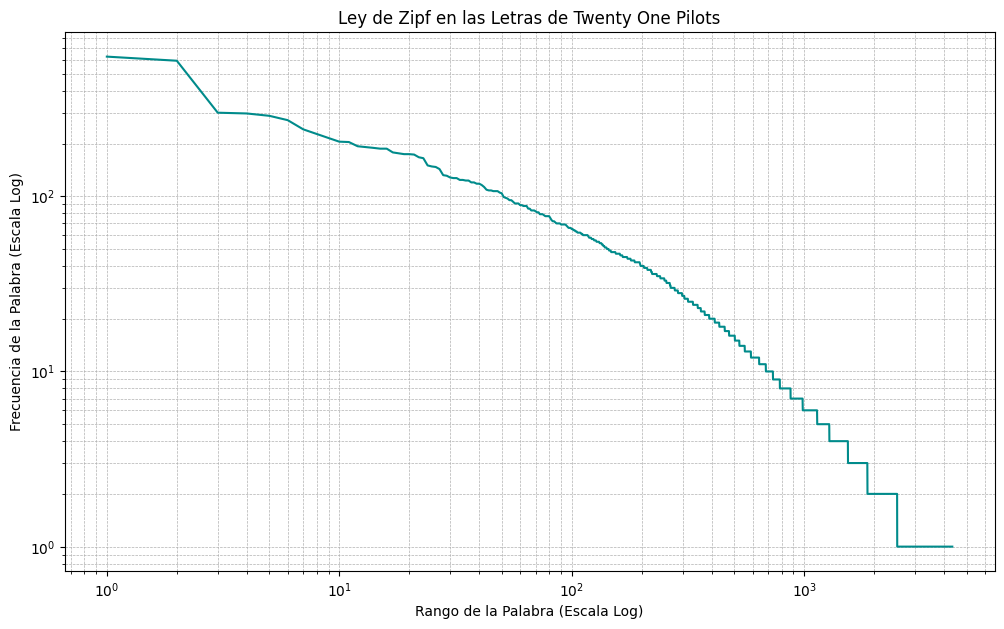
\includegraphics[width=0.8\linewidth]{Images/Zipf_TOP.png}
    \caption{Gráfica de la ley de Zipf para letras de Twenty One Pilots.}
    \label{fig:Zipf_TOP}
\end{figure}

De igual forma, podemos visualizar la frecuencia de las palabras de una manera más artística
implementando una wordcloud. 

\begin{figure}[h!]
    \centering
    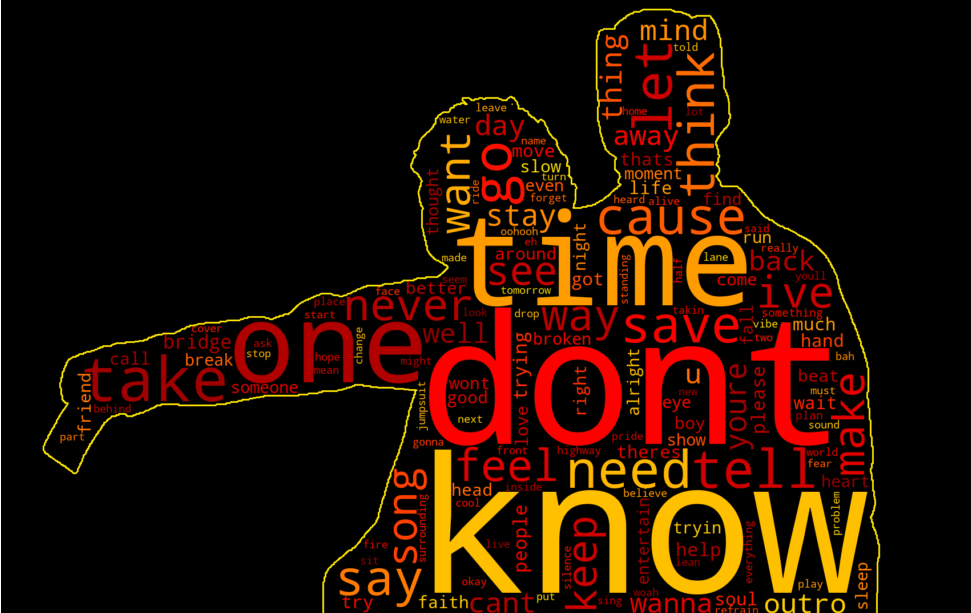
\includegraphics[width=0.8\linewidth]{Images/wordcloud_TOP.png}
    \caption{Wordcloud de Twenty One Pilots.}
    \label{fig:wordcloud_TOP}
\end{figure}

\clearpage





















